\section{Development}
\label{sec:development}

% --------------------------------------------------
\subsection{Code}

JavaScript and Meteor are used on both of the sides, while Node.js is used on the server side, all coded to implement the designed system.
JavaScript is chosen more solely because it is the primary language of the Web.
Meteor is chosen because it is heavily based on JavaScript and easy to learn than any other framework out there.

TODO Some snippets of server-side code

\begin{listing}[htbp]
  \caption{Satellid server code snippets}
  %TODO-CODE \inputminted{javascript}{\dir/include/satellid-server.coffee}
  \label{lst:satellid-code-server}
\end{listing}

TODO Some snippets of client-side code

\begin{listing}[htbp]
  \caption{Satellid client code snippets}
  %TODO-CODE \inputminted{javascript}{\dir/include/satellid-client.coffee}
  \label{lst:satellid-code-client}
\end{listing}

% --------------------------------------------------
\subsection{Result}

TODO Final screenshot

\begin{figure}[htb]
  \centering
  %TODO-SCREEN 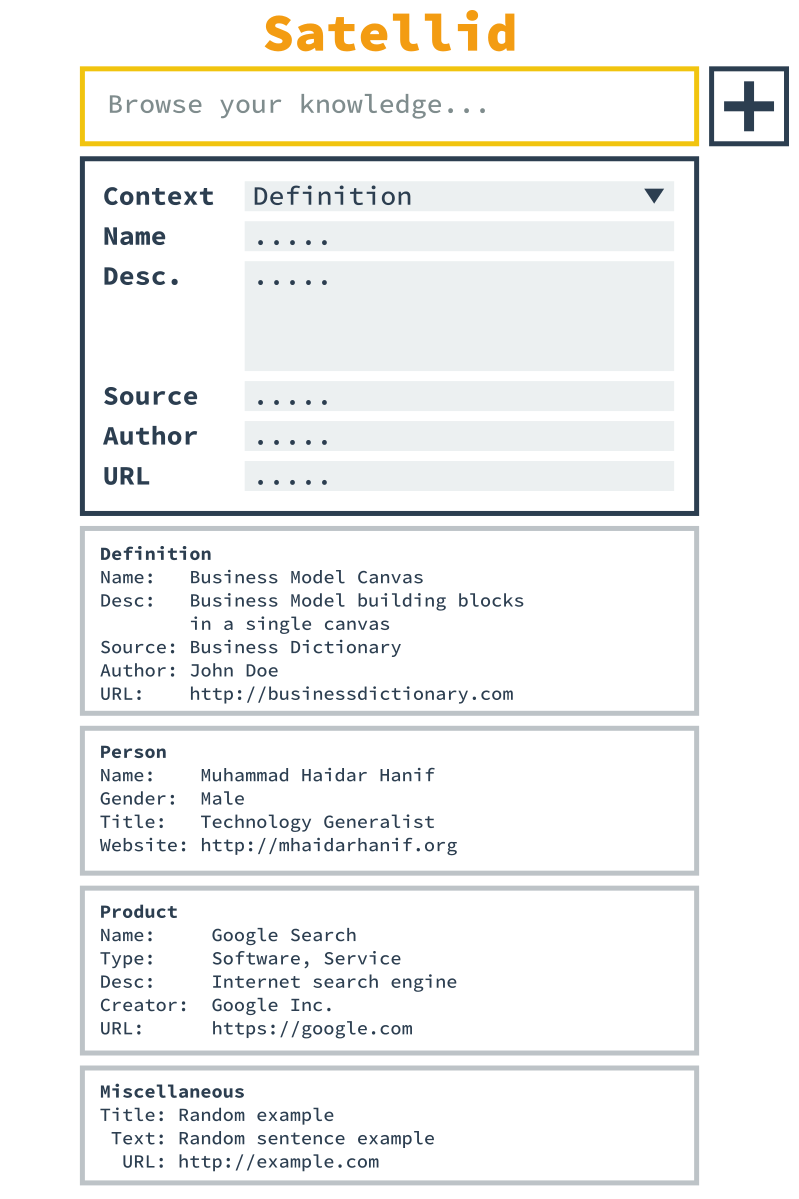
\includegraphics[width=\textwidth]{\dir/include/satellid-result.png}
  \caption{Final screenshot of the development result}
  \label{fig:satellid-result}
\end{figure}
